\documentclass[../template]{subfiles}

\begin{document}
\section{Logica RTL: Transistor Resistor Logic}
Se associamo a valori di tensione alti e bassi (\V{H}, \V{L}) una codifica logica 1 e 0, il circuito precedente si comporta come un invertitore
logico.

Bisogna ricordare che anche il trasporto di carica (corrente) non è uniforme, ed è soggetto anch'esso a rumore.
Il problema che ha questo circuito visto come amplificatore è che amplifica il rumore in ingresso ed il segnale in ingresso dello stesso
fattore $A_V$.
Inoltre dato che il segnale in ingresso varia di poco, la qualità del segnale d'uscita risente molto delle variazioni di rumore.

Diversamente lo stesso circuito visto come invertitore logico, anche a rumore elevato fa il suo lavoro.

L'immunità al rumore è caratterizzato dalle due caratteristiche a guadagno 0 (off e sat). Solo a fronte di valori estremamente alte di rumore, in
grado di entrare nella fascia intermedia, si manifestano sul segnale in uscita.
% 33:00


\subsection{Margine di immunità al rumore}
\begin{figure}[h]
    \centering
    \begin{tikzpicture}[scale=.8]
        \begin{axis}[ymin=-1, xmin=-1, ymax=4]
            \addplot[dashed, clr-gray]{\vcesatval};

            \addplot[domain=-5:\vgamma]{3};
            \addplot[domain=\vgamma:2]{(3 - \vcesatval) / (\vgamma - 2) * x +3 -(3 - \vcesatval) / (\vgamma - 2) * \vgamma };
            \addplot[domain=2:5]{\vcesatval};

            \addplot[dashed, clr-gray] coordinates {(\vgamma, 3) (\vgamma, 0)};
            \draw
                (-0.5, \vcesatval) node[above]{\V{L}}
                (-0.5, 3) node[above] {\V{H}}
                (2, 0) node[below]{\vihmin}
                (3, 0) node[circ]{} node[below]{\V{H}}
                (1.9, 1.9) node[right]{AD}
                (4, \vcesatval) node[above]{SAT}
                (0.4, 3) node[below]{OFF}
                (\vgamma, 0) node[below]{\vilmax}
                ;

        \end{axis}
    \end{tikzpicture}
\end{figure}
\noindent
Dal grafico sono distinguibili un valore basso $\V{L} \equiv \vcesat$, ed un valore alto $\V{H} \equiv \V{cc}$.
La caratteristica da invertitore è esprimibile come $\vu(\V{H}) = \V{L}$ e $\vu(\V{L}) = \V{H}$.
Inoltre siccome questo circuito tollera il rumore, per rumore minore di $\delta_1$ l'uscita \vu sarà ugualmente $\vu(\V{L} + \delta_1) = \V{L}$.
Chiamiamo quindi $\vilmax = \V{L} + \delta_1$ il massimo valore della tensione d'ingresso che produce in uscita un $\V{H}$.
Analogamente chiamo $\vihmin = \V{H} - \delta_2$ il massimo valore della tensione d'ingresso che produce ancora un'uscita $\V{L}$.
Il margine di immunità al rumore \nm è il minimo tra $\delta_1$ e $\delta_2$.
\\
Dato che sappiamo già i valori di \V{H} e \V{L}, calcolando \vihmin come punto di intersezione tra la zona attiva diretta e di saturazione,
otteniamo:
\begin{align*}
    \delta_1 = \vilmax - \V{L} = \vgamma - \vcesatval = 0.55 V\\
    \delta_2 = \V{H} - \vihmin = 5 - 1.23 = 3.77V
\end{align*}
Da cui $\nm = 0.55 V$. Per avere immunità al rumore è necessario che $\delta_1 = \vilmax - \V{L}$ e $\delta_2 = \V{H} - \vihmin$ siano positivi
sarà positiva anche la loro somma, per questo possiamo dire che
\begin{align*}
    \V{H} - \V{L} > \vihmin - \vilmax\\
    \frac{\V{H} - \V{L}}{ \vihmin - \vilmax} > 1
\end{align*}
Facendo sempre riferimento al grafico è facile capire che rapporto tra $\V{H} - \V{L}$ e $\vihmin - \vilmax$ è $|A_V|$.
Per cui $|A_V| > 1$. Maggiore sarà il valore di $|A_V|$, migliore è la proprietà di filtro per il rumore di questo
circuito.

Il risultato ottenuto dipende fortemente dall'approssimazione lineare utilizzata, dato il valore alto \V{H} ed il valore
basso \V{L} sono stati definiti graficamente, in corrispondenza di \V{cc} e \vcesat.
Generalizziamo quindi questa definizione facendo riferimento ad altri circuiti.

Preso un andamento di circuito generico (es. figura \ref{fig:bjt_graph}) rimane ancora vero che esistono due regioni con
guadagno basso ed una con guadagno maggiore di 1, ma la distinzione di \V{H} e \V{L} non è ovvia come nel caso
precedente.


Per identificare il valore di \vl e \vh, facciamo il seguente ragionamento:
considerando una serie di $n$ invertitori, l'andamento del valore di uscita sarà identico per tutti gli invertitori di
posto pari, mentre sarà invertito per tutti gli invertitori di posto dispari.
Dato che gli invertitori di posto dispari dovranno corrispondere alla funzione inversa degli invertitori di posto pari,
il loro grafico è uguale al grafico degli invertitori di posto pari ma specchiato rispetto alla bisettrice.
\begin{figure}[h]
    \centering
    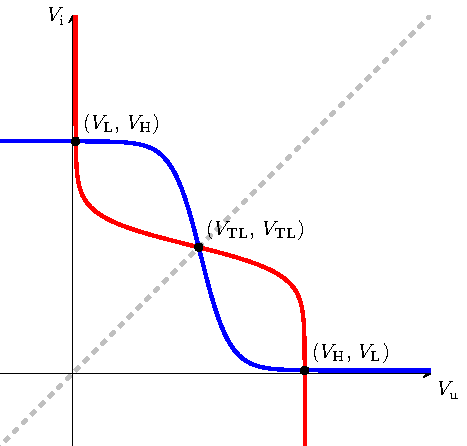
\includegraphics[width=2in]{graph_double_not}
    \caption{Grafico}
    \label{fig:graph_double_not}
\end{figure}

Siccome è ovvio che quando tutti gli invertitori sono connessi in cascata, le loro condizioni devono essere soddisfatte,
esistono solo 3 punti in queste caratteristiche che soddisfano le equazioni (vedi figura \ref{fig:graph_double_not}).
Le coppie di punti $(\vl, \vh)$ e $(\vh, \vl)$ sono simmetrici per costruzione, per questo sono i valori \vh e \vl che
stavamo cercando.

Definiamo questo punto l'escursione logica \ls (\textit{Logic Swing}) come $\vh - \vl$.

Il punto $(\vtl, \vtl)$ è tale per cui se posto in ingresso al primo invertitore, si propaga invariato fino al termine
della catena. In realtà questa condizione è quasi impossibile, siccome ci troviamo in una zona con $|A_V| > 1$
ed al primo segnale di rumore veniamo spostati verso \vh o \vl, allontanandoci dal punto di precario equilibrio, detto
anche metastabile.

Possiamo osservare che la qualità (intesa come distanza da \vh o \vl), aumenta, lungo la catena di invertitori. Questa
proprietà prende il nome di \textbf{proprietà rigenerativa del segnale}.

Per questo motivo, osservando anche in ingresso un valore compreso in un intorno di \vl, per la proprietà appena citata,
esso viene trattato ugualmente come valore nominale basso. Il valore \vtl si comporta quindi come soglia logica,
discriminando i valori alti dai valori bassi.
% Esempio palline 30:50 lez 11

Questa proprietà è strettamente legata alla disuguaglianza $|A_V| > 1$. Nel caso quest'ultima non fosse verificata,
osserviamo che il punto di intersezione delle due caratteristiche è uno solo (vedi figura da fare)

\begin{figure}[h]
    \centering
    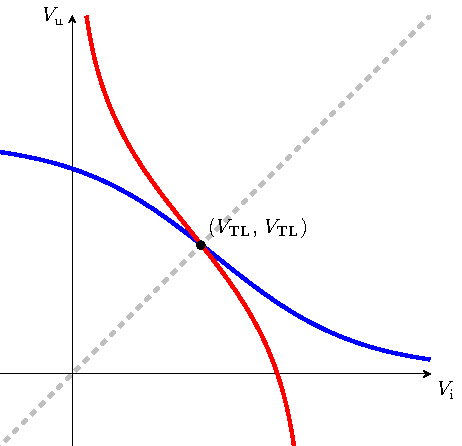
\includegraphics[width=2in]{graph_not_a_low}
    \caption{grafico per $|A_V| < 1$}
\end{figure}

Quindi in caso $|A_V| < 1$ ogni punto in ingresso alla catena di invertitori, convergerebbe in $(\vtl, \vtl)$.
\newpage
\subsubsection{Margine di immunità ai disturbi}
Rimane comunque vero che se il guadagno è minore di 1, il rumore in uscita è minore del rumore in ingresso, mentre se il
guadagno è maggiore di 1, il rumore in ingresso è amplificato.  Possiamo quindi identificare due punti, con guadagno
$|A_V| = 1$, per suddividere i tratti di caratteristica, identificati da $|A_V| < 1$ e $|A_V| > 1$.

Utilizzando la stessa nomenclatura della logica RTL, chiamiamo \vilmax, il punto per cui il tratto $0 < x < \vilmax$ ha
$|A_V| < 1$, e \vihmin il tratto in cui $\vihmin < x$ per cui $|A_V| < 1$. Di conseguenza $\vilmax < x < \vihmin$ è
caratterizzato da $|A_V| > 1$.


Indichiamo inoltre con $\vohmin = \vu(\vilmax)$ il più piccolo valore dell'uscita associato all'attenuazione
del rumore. Analogamente $\volmax=\vu(\vilmax)$.

\begin{figure}[h]
    \centering
    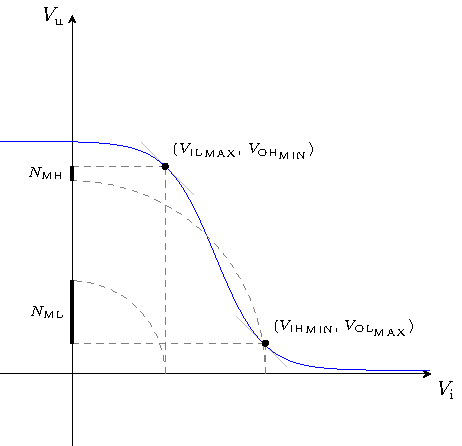
\includegraphics{graph_margine_soglia}
\end{figure}

La massima quantità di rumore accettabile per non uscire dalla regione di attenuazione sono $N_H = \vohmin - \vihmin$ e
$N_L = \vilmax - \volmax$. Quindi $N_M = \min(\vohmin - \vihmin, \vilmax - \volmax)$.
% Grafico 57
Da questa costruzione risulta evidente che $\ls > N_H + N_L$, quindi nel caso in cui una delle due soglie sia
controllata (ad esempio da una resistenza variabile) e dovesse aumentare di valore, l'altra sarebbe costretta a
diminuire, per evitare che la somma superi \ls.

La condizione ottimale per avere massimo margine ai disturbi è quindi in caso in cui $N_L$ e $N_H$ siano simmetrici.
(nel caso di approssimazione i punti coincidono con vh e vl, dato che per approssimazione non ci sono punti con derivata
= -1, passa dal valore in modulo < 1 a modulo > 1)

\newpage
\subsection{Porta logica NOR}
\begin{figure}[h]
    \centering
    \begin{circuitikz}
        \draw (0, 0)
        node[above] {$V_{i1}$}
        to[R, l=$R_B$, i=$I_B$, *-] (2,0)
        node[npn, anchor=B](tl){}


        (tl.C) to[short,] ++(2,0)
        node[npn, anchor=C, xscale=-1](tr){}

        (tl.C) ++(1, 0) node[circ]{}
        node[below]{$V_u$}
        to[R, l=$R_C$, i<=$I_{RC}$] ++(0, 2)
        node[vcc]{} node[right]{$V_{cc}$}

        (tr.B) to[R, l=$R_B$, i<=$I_B$, -*] ++(2, 0)
        node[above]{$V_{i2}$}
        (tl.E) node[ground]{}
        (tr.E) node[ground]{}

        (tl) node[right]{$T_1$}
        (tr) node[left]{$T_2$}
        ;
    \end{circuitikz}
\end{figure}

Supponendo i valori delle resistenze $R_C = 1k\Omega$ e $R_B = 10k\Omega$, e $\beta_F = 100$
vogliamo valutare il comportamento di questa rete al variare dei due ingressi $V_{i1}$ e $V_{i2}$, prendendo il caso di segnali in ingresso digitali:
$\vi = \{\vh, \vl\}$.
Le combinazioni possibili in ingresso sono quindi enumerabili e studiabili individualmente.
\begin{tcolorbox}[title=Equazioni Generali]
    \begin{align*}
        &\I{RC} = \I{C1} + \I{C2}\\
        &\vi - R_B \I{B} - \vbe = 0
    \end{align*}
\end{tcolorbox}
Nel caso di un qualsiasi transistore spento, considerando che $\vbe < V_\gamma$ per ipotesi, otteniamo $\vi < V_\gamma$.
\begin{tcolorbox}[title={Per ${\vi}_1 = {\vi}_2 = \vl$}]
    \begin{align*}
        \vi < V_\gamma\\
        \vu = \V{cc}
    \end{align*}
\end{tcolorbox}
\begin{tcolorbox}[title={Per ${\vi}_1 \vl, {\vi}_2 = \vh$}]
    Osservando l'alta tensione ricevuta all'ingresso, è ragionevole ipotizzare che $T_2$ si trovi in regime di funzionamento saturo.
    Verificando quindi le ipotesi:
    \begin{align*}
        &\I{B} = \frac{\V{cc} - V_\gamma}{R_B} = 0.425mA > 0\\
        &\I{C} = \frac{\V{cc} - \vcesat}{R_C} = 4.8 mA < \beta_F \I{B} = 42.5mA\\
    \end{align*}
    Per cui in questo caso $\vu = \vcesat = \vl$
\end{tcolorbox}
\begin{tcolorbox}[title={Per ${\vi}_1 = {\vi}_2 = \vh$}]
    Per ragionamento analogo al caso precedente, ci aspettiamo che entrambi i transistori siano saturi. Quindi $\vu = \vcesat = \vl$
    \begin{align*}
        &\I{B} = \frac{\V{cc} - V_\gamma}{R_B} = 0.425mA > 0\\
        &\I{RC} = \frac{\V{cc} - \vcesat}{R_C} = 4.8 mA < \beta_F \I{B} = 42.5mA\\
    \end{align*}
    Essendo il circuito perfettamente simmetrico non c'è motivo di ipotizzare che $\I{C1} \neq \I{C2}$. Per cui $\I{C1} = \I{C2} = 4.8mA$,
    quindi sono verificate entrambe le condizioni $\I{C} < \beta_F \I{B}$.
\end{tcolorbox}
Questa rete si comporta come una porta logica NOR.
La rete composta dai transistori $T_1$ e $T_2$ è definita come \textbf{rete di pulldown}, ovvero quando è accesa, trascina il valore di uscita verso il valore basso.
Analogamente è possibile interpretare la rete composta dalla resistenza $R_c$ come una \textbf{rete di pullup}: quando non è contrastata da reti di pulldown attive, l'uscita viene portata a \vh da $R_c$ dove non circola corrente.

Osserviamo che questo circuito si comporta allo stesso modo se alla rete di pulldown è composta da più di due transistori, dato che la corrente $\I{RC}$ sarebbe suddivisa equamente tra tutti i transistori accesi, mantenendo vera l'ipotesi $\I{C} < \beta_F \I{B}$. Quindi questo circuito è generalizzabile ad una porta NOR a numero arbitrario di ingressi.

L'insieme degli ingressi prende il nome di \textit{fan-in}, mentre il numero di uscite prende il nome di \textit{fan-out}.
Siccome l'operatore NOR è una famiglia funzionalmente completa, con la logica RTl è possibile realizzare una qualsiasi funzione combinatoria.

Manca da analizzare se la connessione in serie delle seguenti porte NOR, mantenga il valore del segnale.

\begin{figure}[h]
    \centering
    \begin{circuitikz}
        \draw(0, 0)
        % First transistor
        node[circ]{} node[left]{$V_i$}
        to[R, l=$R_B$] ++(1.5, 0)
        node[npn, anchor=B] (n1) {}

        (n1.C) to[R] ++(0, 1.5) node[vcc]{}
        (n1.E) node[ground]{}

        % First transistor label
        (n1) node[right]{$T$}

        % Connect Vu1 to Vi2
        (n1.C) -- ++(1, 0) -| (4, 0)

        % Second transistor
        node[circ]{} node[below]{$V_u' = V_i$'}
        to[R, l=$R_B$] ++(1.5, 0)
        node[npn, anchor=B] (n2) {}

       (n2.C) to[R] ++(0, 1.5) node[vcc]{}
        (n2.E) node[ground]{}

        % Second transistor label
        (n2) node[right]{$T'$}

        % Draw Vu
        (n2.C) -- ++(0.5, 0) node[circ]{} node[right]{$V_u$}
        ;
    \end{circuitikz}
\end{figure}
\begin{tcolorbox}[title={$T$ OFF }]
Partendo ad analizzare la condizione per cui $T$ OFF otteniamo che $\vu = \V{cc} - R_C \I{B}$
Nel caso in cui anche $T'$ sia OFF, allora $\I{B}'$ è 0 e di conseguenza:
\begin{align*}
    &\vu = \V{cc}\\
    &\vi' -\cancel{R\I{B}'} = \vbe'
\end{align*}
Ma ciò non è possibile dato che se $T'$ è OFF, allora $\vbe' < V_\gamma$. Quindi $T'$ non può essere OFF se $T$ è OFF.
Quindi $T'$ è necessariamente acceso, con $\vbe'=V_\gamma$. Dall'equazione di kirkoff al nodo \vu:
\[
    \frac{\V{cc} - \vu}{R_C} = \frac{\vu - V_\gamma}{R_B}
\]
Ottenendo $\vu = \frac{R_B \V{CC} + R_C V_\gamma}{R_B + R_C} = < V_\gamma$ svolgendo la disequazione si ottiene: $V_\gamma < \V{cc}$.
Sostituendo inoltre i dati utilizzati nel circuito precedente, otteniamo $\vu = 4.61V$
\end{tcolorbox}

\begin{tcolorbox}[title={$T$ in AD}]
    \[
        \vu = \V{cc} - R_C \Big\{\beta_f \frac{\vi - V_\gamma}{R_B} + \frac{\vu - V_\gamma}{R_B}\Big\}
    \]
    Da cui
    \[
        \vu = {\color{clr-primary} \frac{R_B \V{cc} + R_C V_\gamma}{R_B + R_C}} - {\color{red}\frac{\beta_F R_C}{R_B + R_C}}(\vi - V_\gamma)
    \]
    Osserviamo come il termine blu è identico a quello calcolato in precedenza, nel tratto di regione attiva diretta, mentre il tratto rosso è un guadagno di modulo minore rispetto a quello di prima ($\frac{\beta_F R_C}{R_B}$).

    Questa condizione è valida fino a quando o $T$ passa alla regione di saturazione ($\vu=\vcesat$) o $T'$ passa in regione attiva diretta ($\vu = V_\gamma$).
    Dato che $\vu < V_\gamma$ avverrà prima, sostituendo tale valore nell'equazione di \vu segue $\vi = 1.175V$
\end{tcolorbox}
\begin{tcolorbox}[title={$T$ in AD e $T'$ OFF}]
    Questo tratto di caratteristica corrisponde esattamente al precedente.
\end{tcolorbox}

\begin{tikzpicture}
    \def\rc{80}
    \def\rb{400}
    \def\betaf{30}

    \begin{axis}[ymax=6, ymin=-1, xmin=-1]
        \addplot[thin, red, domain=-5:\vgamma]{(\rb * 5 + \rc * \vgamma)/(\rb + \rc)};
        \addplot[thin, red, domain=\vgamma:{-(\vgamma - (\rb * 5 + \rc *\vgamma)/(\rb + \rc))*((\rb + \rc)/(\betaf*\rc)) + \vgamma}]{(\rb * 5 + \rc * \vgamma)/(\rb + \rc) - (\betaf*\rc)/(\rb + \rc) * (x - \vgamma)};
        \addplot[thin, red, domain={-(\vgamma - (\rb * 5 + \rc *\vgamma)/(\rb + \rc))*((\rb + \rc)/(\betaf*\rc)) + \vgamma}:{(5 - \vcesatval)*\rb/(\betaf*\rc) + \vgamma}]{5 - \betaf*\rc/\rb*(x - \vgamma)};

        \addplot[thin, black, domain=-5:\vgamma]{5};
        \addplot[thin, black, domain=\vgamma:{(5 - \vcesatval)*\rb/(\betaf*\rc) + \vgamma}]{5 - \betaf*\rc/\rb*(x - \vgamma)};
        \addplot[thin, black, domain={(5 - \vcesatval)*\rb/(\betaf*\rc) + \vgamma}:5]{\vcesatval};

        \addplot[thin, lightgray, dashed] coordinates {(\vgamma, 0) (\vgamma, 5)};
        \addplot[thin, lightgray, dashed, domain=0:{-(\vgamma - (\rb * 5 + \rc *\vgamma)/(\rb + \rc))*((\rb + \rc)/(\betaf*\rc)) + \vgamma}] {\vgamma};
        \draw (\vgamma, 0) node[below] {$V_\gamma$}
              (0, \vgamma) node[left]{$V_\gamma$};

        \draw (\vgamma, 5) node[circ]{}
            node[anchor=south west]{\scriptsize $(\vilmax, \vohmin)$}
            ({(5 - \vcesatval)*\rb/(\betaf*\rc) + \vgamma}, \vcesatval) node[circ]{}
            node[anchor=south west]{\scriptsize $(\vihmin, \volmax)$}
            ;
    \end{axis}
\end{tikzpicture}

Delle quattro coordinate utilizzate per calcolare il margine di rumore, solo una è modificata dal fatto che il FAN-OUT è modificato da 0 a 1.
Il margine $\nml$ definito quindi per il livello basso rimane invariato: $\nml = \vilmax - \volmax = V_\gamma - \vcesat = 0.55 V$.
Diversamente il margine $\nmh$ varia: $\nmh = \vohmin - \vihmin = 4.61 - 1.23 = 3.37V$.

Il margine complessivo, rimanendo definito come il minimo tra $\nml$ e $\nmh$ rimane invariato a $0.55V$.

Nel caso di un FAN-OUT generico ad $n$ porte il valore $\nmh$ tenderà a calare, dato che, la corrente del transitorio di pullup è richiamata dagli altri componenti connessi.

Generalizzando con $n$ componenti connessi che condividono \vu come tensione in ingresso, dato che tutti hanno la stessa \vi, tutti i transistori si troveranno nella stessa regione di funzionamento. Quindi le correnti in ingresso $\I{B}$ necessariamente coincidono quindi $\I{RC} = \I{C} + n \I{B}'$.

Nell'ipotesi che il transistore $T$ sia spento:
\begin{align*}
    &\I{RC} = \frac{\V{cc} - \vu}{R_C} \\
    &\I{B}' = \frac{\vu - V_\gamma}{R_B}
\end{align*}
Ottenendo la generica relazione:
\[
    \vu(n) = \vohmin(n) = \frac{R_B \V{cc} + n R_C V_\gamma}{R_B + n R_C}
\]
Da cui $\nmh = \vohmin(n) - 1.23$. Definiamo con FAN-OUTmax il massimo punto in per cui il valore di $\nmh$ rimane superiore a $\nml$.
Risolvendo l'equazione $0.55 = \vohmin(n) - 1.23$ otteniamo $n = 31.26$, per questo FAN-OUTmax è 31.
\end{document}
